\section{Results}\label{sec:results}

All numbers are full-wave CST simulation under position-grouped 5-fold CV. The
headline CFM posterior and point numbers are on the combined $N=3935$ set; the
multi-method uncertainty comparison (Table~\ref{tab:uq}) is on the
initial-stage subset ($N=1980$) and is labelled as such. The headline result is
calibration with discrimination: the CFM posterior is the only evaluated method
that clears point error, multi-level coverage, and error--spread ranking
together, while preserving backbone-level point accuracy within seed variation.
We report the point-accuracy reference first (Section~\ref{sec:res-point}),
then the calibration result (Section~\ref{sec:res-uq}), the deployability
ablation (Section~\ref{sec:res-deploy}), a controlled observability probe of
posterior modality (Section~\ref{sec:res-modality}), and the
orientation-marginal width result (Section~\ref{sec:res-orient}).

\subsection{Point accuracy: the posterior preserves backbone accuracy within seed variation}\label{sec:res-point}
Table~\ref{tab:point} supports the point-cost claim on the combined $N=3935$
rich set. The clean
CFM posterior (\SI{0.354}{cm}, 95\% CI $[0.339,0.369]$) ties the deterministic
backbone (\SI{0.340(4)}{cm} on the combined $N=3935$ set; \SI{0.340}{cm} in
Table~\ref{tab:point}) within seed noise and significantly outperforms all ten
classical regressors: every position-paired 95\% bootstrap interval on the
difference excludes zero, with the best classical method (HistGradientBoosting,
\SI{0.779}{cm}) trailing CFM by $+\SI{0.424}{cm}$ $[0.405,0.443]$. The
deterministic backbone's per-axis errors are $x/y/z =
0.14/0.17/0.18\SI{}{cm}$; the per-axis CFM error is balanced ($x/y/z =
0.143/0.181/0.185\SI{}{cm}$). On the corrected geometry the $y$ axis is no
longer the entire error budget. The CFM-vs-backbone
tie lacks a paired CI because the backbone's per-point predictions were not
retained; we therefore report it as ``within seed noise,'' not as a significance
test. Figure~\ref{fig:point-ranking} shows that CFM preserves backbone-level
point accuracy while beating the classical regressors, Figure~\ref{fig:peraxis}
confirms the corrected geometry balances the axes, and
Figure~\ref{fig:hero-grid} shows that the residual error is concentrated on the
no-face-coverage $y$ axis.

\begin{figure}[t]
\centering
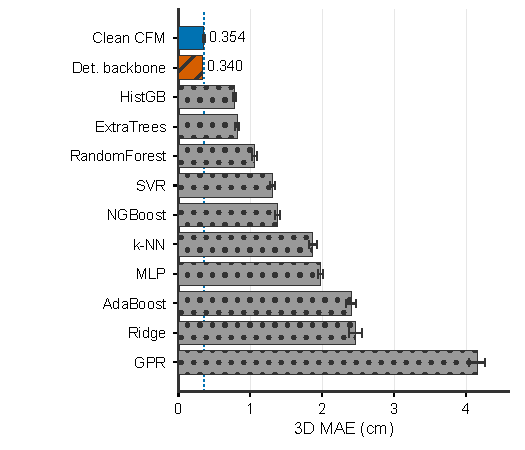
\includegraphics[width=0.9\linewidth]{figures/fig_point_ranking.pdf}
\caption{Point-accuracy ranking on the combined rich set ($N=3935$). Horizontal
bars show 3D MAE; error bars show position-paired 95\% bootstrap CIs where
available. Clean CFM ties the deterministic backbone within seed noise and
outperforms the classical regressors under identical position-grouped folds.
\textbf{Simulation.}}
\label{fig:point-ranking}
\end{figure}

\begin{figure}[t]
\centering
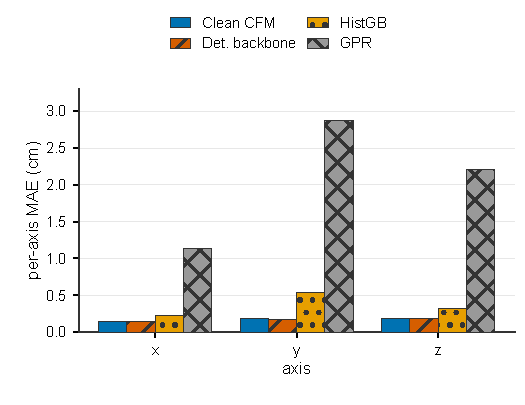
\includegraphics[width=0.9\linewidth]{figures/fig_peraxis.pdf}
\caption{Per-axis MAE on the combined rich set ($N=3935$). The anti-symmetric
receiver placement leaves $y$ as the hardest axis but breaks the mirror symmetry enough
for CFM and the deterministic backbone to remain balanced; GPR is dominated by
$y$ error. \textbf{Simulation.}}
\label{fig:peraxis}
\end{figure}

\begin{figure*}[t]
\centering
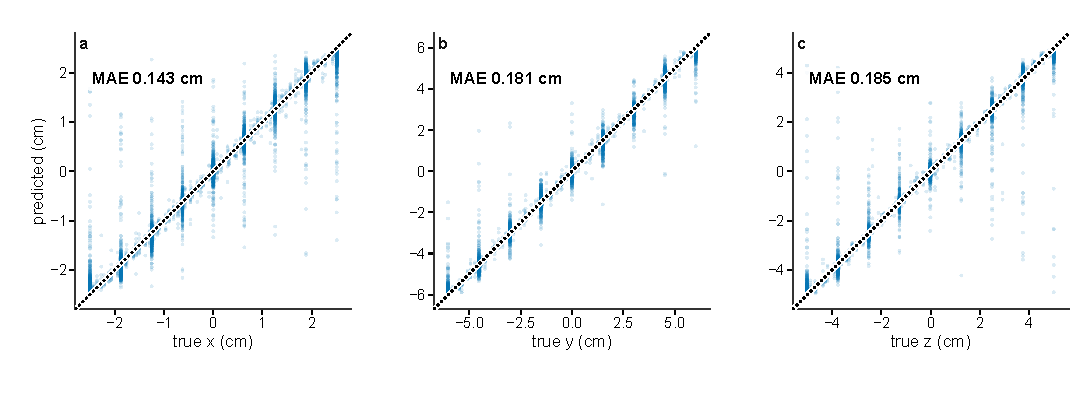
\includegraphics[width=0.96\linewidth]{figures/fig_hero_grid.pdf}
\caption{CFM predicted versus true position per axis on the combined set
($N=3935$); points on the dotted identity line are exact. The $x$ and $z$ axes are
tightly recovered, while $y$---the axis with no face receivers---carries most of
the residual error, consistent with Fig.~\ref{fig:peraxis}. \textbf{Simulation.}}
\label{fig:hero-grid}
\end{figure*}

\begin{table}[t]
\centering
\caption{Point accuracy on the combined rich set ($N=3935$, position-grouped
5-fold CV, 3 seeds), 3D MAE with position-paired 95\% bootstrap CIs (paired vs.\
CFM over the 788 unique positions). \textbf{Simulation.}}
\label{tab:point}
\scriptsize
\setlength{\tabcolsep}{3pt}
\begin{tabular}{lcc}
\toprule
Method & 3D MAE (cm) & Paired $\Delta$ vs.\ CFM (cm) \\
\midrule
Deterministic backbone (point ref.) & 0.340 & tie\,$^{\dagger}$ \\
\textbf{Clean CFM (posterior mean)} & \textbf{0.354}\;[0.339,0.369] & --- \\
\midrule
HistGradientBoosting & 0.779\;[0.756,0.801] & $+0.424\;[0.405,0.443]$ \\
ExtraTrees           & 0.817\;[0.788,0.845] & $+0.462\;[0.439,0.486]$ \\
RandomForest         & 1.061\;[1.026,1.095] & $+0.706\;[0.677,0.735]$ \\
SVR                  & 1.306\;[1.267,1.342] & $+0.952\;[0.920,0.983]$ \\
NGBoost              & 1.382\;[1.346,1.417] & $+1.028\;[0.994,1.060]$ \\
$k$-Neighbors        & 1.869\;[1.813,1.923] & $+1.515\;[1.462,1.565]$ \\
MLPRegressor         & 1.978\;[1.941,2.012] & $+1.624\;[1.592,1.652]$ \\
AdaBoost             & 2.404\;[2.334,2.474] & $+2.052\;[1.984,2.116]$ \\
Ridge                & 2.460\;[2.377,2.553] & $+2.108\;[2.026,2.194]$ \\
GPR (fixed kernel)   & 4.153\;[4.037,4.266] & $+3.800\;[3.687,3.908]$ \\
\bottomrule
\end{tabular}
\\[2pt]
{\footnotesize $^{\dagger}$Tie within seed noise; paired CI not available because
the backbone per-point predictions were not retained for this analysis. All values are
full-wave CST simulation under position-grouped 5-fold CV.}
\end{table}

\subsection{Calibration: the only method clearing all three bars}\label{sec:res-uq}
Table~\ref{tab:uq} is the central result. In the multi-method comparison on the
initial-stage subset ($N=1980$), the clean CFM posterior is the \emph{only}
method that
simultaneously achieves competitive point error, coverage from its own samples
that is \emph{conservative} at the 50\% level and near-nominal at 90/95\%
(marginal 50/90/95\% $=0.766/0.935/0.944$), and real error--spread
discrimination ($\rho=0.601$). The deep ensemble attains marginally lower MAE
(\SI{0.359}{cm}) and higher $\rho$ ($0.705$) but \emph{under-covers} badly
(cov$_{90}=0.717$); MC-dropout under-covers severely (cov$_{90}=0.464$). Both
mixture-density networks \emph{over-cover} (cov$_{90}\approx0.96$--$0.97$) with
near-zero discrimination ($\rho\le0.10$): they widen without ranking.
Split conformal targets nominal coverage; its observed cov$_{90}=0.893$ and it
likewise carries $\rho\approx0$. On the full combined $N=3935$ set the CFM posterior is
consistent and slightly conservative (marginal 50/90/95\% $=0.832/0.970/0.975$;
joint $0.624/0.925/0.939$; pooled $\rho=0.58$, fold-mean $0.62$; CRPS
\SI{0.127}{cm}, energy score \SI{0.277}{cm}, sharpness \SI{0.281}{cm};
Fig.~\ref{fig:crps}).
The deterministic backbone produces no posterior. Of the classical regressors,
only NGBoost and the fixed-kernel Gaussian process emit a predictive variance,
but both are \emph{parametric and unimodal}---they cannot represent the
multimodality that is the point of Section~\ref{sec:res-modality}---and their
point error (Table~\ref{tab:point}) is far from the operating region of interest;
we therefore restrict the uncertainty panel to the sampling-based posteriors and
the conformal baseline. Figure~\ref{fig:cal-disc} shows that only CFM occupies
the near-nominal, high-discrimination region, Figure~\ref{fig:reliability}
confirms the multi-level coverage pattern, and Figure~\ref{fig:error-spread}
shows that CFM spread ranks realized error on the combined set. Because the spread
ranks error, deferring the least-confident estimates sharply reduces the error of
the retained set---at $50\%$ retention the 3D MAE falls from \SI{0.354}{cm} to
${\sim}\SI{0.18}{cm}$, tracking the oracle ordering (Fig.~\ref{fig:risk-coverage})---which
is the basis for a selective-prediction operating point.

\begin{figure}[t]
\centering
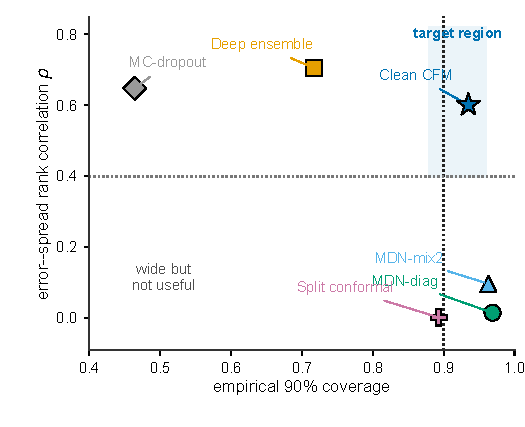
\includegraphics[width=0.9\linewidth]{figures/fig_cal_vs_disc.pdf}
\caption{Calibration versus discrimination in the initial-stage subset
($N=1980$). The horizontal axis is empirical 90\% coverage and the
vertical axis is Spearman error--spread correlation; CFM is the only method in
the near-nominal, high-discrimination region. \textbf{Simulation.}}
\label{fig:cal-disc}
\end{figure}

\begin{table}[t]
\centering
\caption{UQ bake-off on the \textbf{initial-stage subset ($N=1980$)}, marginal
coverage. \textbf{Bold} = the only method clearing point + near-nominal coverage
+ discrimination together. \textbf{Simulation.}}
\label{tab:uq}
\setlength{\tabcolsep}{3.5pt}
\begin{tabular}{lccccc}
\toprule
Method & MAE & cov$_{50}$ & cov$_{90}$ & cov$_{95}$ & $\rho_{\text{err,spread}}$ \\
       & (cm) & & & & \\
\midrule
\textbf{Clean CFM} & \textbf{0.501} & \textbf{0.766} & \textbf{0.935} & \textbf{0.944} & \textbf{0.601} \\
Deep ensemble (5)  & 0.359 & 0.402 & 0.717 & 0.738 & 0.705 \\
MC-dropout (50)    & 0.473 & 0.206 & 0.464 & 0.523 & 0.648 \\
MDN-diag (200)     & 0.533 & 0.874 & 0.969 & 0.978 & 0.015 \\
MDN-mix2 (200)     & 0.614 & 0.837 & 0.963 & 0.973 & 0.097 \\
Split conformal    & ---   & 0.483 & 0.893 & 0.945 & 0.002 \\
\bottomrule
\end{tabular}
\\[2pt]
{\footnotesize All values are full-wave CST simulation under position-grouped
5-fold CV. Split conformal wraps the deterministic backbone's point estimate;
its point MAE is therefore not repeated. Combined-set CFM-only values are
reported in the text.}
\end{table}

\begin{figure}[t]
\centering
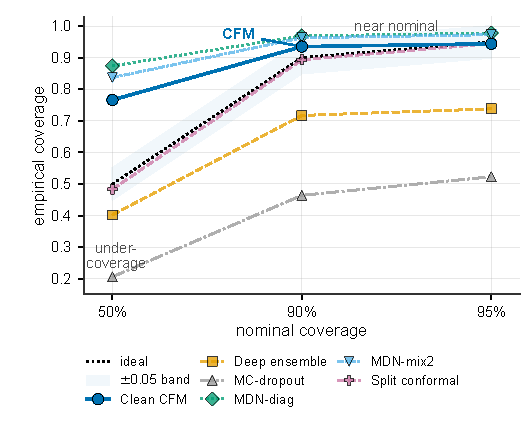
\includegraphics[width=0.86\linewidth]{figures/fig_reliability.pdf}
\caption{Coverage reliability on the initial-stage subset ($N=1980$), marginal.
Clean CFM is
conservative at the 50\% level and close to the diagonal at 90/95\%; the deep
ensemble and MC-dropout under-cover; the MDNs over-cover.
Combined-set CFM is slightly conservative (text). \textbf{Simulation.}}
\label{fig:reliability}
\end{figure}

\begin{figure}[t]
\centering
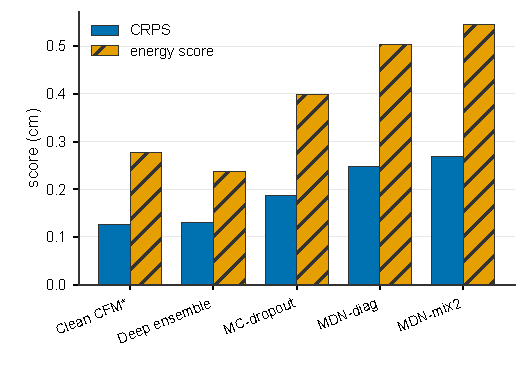
\includegraphics[width=0.92\linewidth]{figures/fig_crps.pdf}
\caption{Proper scoring rules (lower is better): CRPS and energy score per method.
CFM$^{*}$ is scored on the combined set while the other methods use the
initial-stage subset ($N=1980$, as
in Table~\ref{tab:uq}), so the bars are \emph{not} directly comparable; on its
own set CFM attains a low CRPS and a competitive energy score. \textbf{Simulation.}}
\label{fig:crps}
\end{figure}

\begin{figure}[t]
\centering
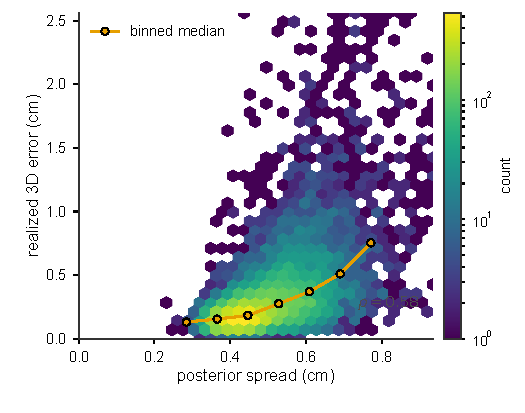
\includegraphics[width=0.9\linewidth]{figures/fig_error_spread.pdf}
\caption{Per-point CFM error versus posterior spread on the combined set
($N=3935$). Each point is a held-out configuration; the positive rank correlation
shows that the posterior width is useful for selective prediction, not merely
wider on average. \textbf{Simulation.}}
\label{fig:error-spread}
\end{figure}

\begin{figure}[t]
\centering
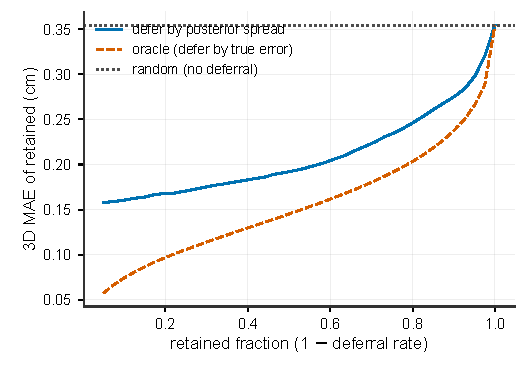
\includegraphics[width=0.9\linewidth]{figures/fig_risk_coverage.pdf}
\caption{Selective prediction on the combined set ($N=3935$). Deferring the
least-confident estimates by posterior spread (solid) monotonically lowers the
3D MAE of the retained set and closely tracks the oracle ordering by true error
(dashed); the dotted line is the no-deferral mean. The gap between the spread and
oracle curves is the residual room for a better confidence signal.
\textbf{Simulation.}}
\label{fig:risk-coverage}
\end{figure}

\subsection{Deployability ablation: RF phase, not bandwidth, is the lever}\label{sec:res-deploy}
A single-tone magnitude-only MICS/MedRadio device cannot measure phase, so
Table~\ref{tab:deploy} and Figure~\ref{fig:deployability} ablate which feature
components drive sub-cm accuracy on the initial-stage subset ($N=1980$). This
single-tone magnitude-only ablation is the strict-legal-band evidence. The
\emph{single-tone, magnitude-only} floor (S1) is
${\sim}\SI{1.5}{cm}$ (CFM \SI{1.519}{cm}, HistGB \SI{1.550}{cm}, ExtraTrees
\SI{1.731}{cm}). Adding phase at a single tone (S2) drops HistGB to
\SI{0.970}{cm} ($-37\%$) and CFM to \SI{0.524}{cm}; recovering phase across the
coherent sub-band ${\sim}$\SIrange{402}{405}{MHz} (S3) reaches CFM
\SI{0.481}{cm}, matching the full rich
representation on the same subset (S5, CFM \SI{0.512}{cm}). Crucially,
\emph{multi-frequency magnitude alone} (S4) does \emph{not} reach the
sub-centimetre regime (CFM \SI{1.191}{cm}, HistGB \SI{1.652}{cm}): bandwidth
without phase coherence is not enough. The deployable magnitude-only number to
quote is ${\sim}\SI{1.5}{cm}$; sub-centimetre accuracy requires phase-coherent
receivers. Because this ablation uses the smaller initial-stage subset
($N=1980$), the S5 CFM value should not be compared directly with the
combined-set CFM headline in Table~\ref{tab:point}.

\begin{table}[t]
\centering
\caption{Feature-deployability ablation on the \textbf{initial-stage subset
($N=1980$)}
(3D MAE, cm). Phase coherence (S2/S3/S5), not bandwidth alone (S4),
separates the ${\sim}\SI{1.5}{cm}$ single-tone floor from the sub-cm regime.
\textbf{Simulation.}}
\label{tab:deploy}
\setlength{\tabcolsep}{4pt}
\begin{tabular}{llccc}
\toprule
& Feature set & HistGB & ExtraTrees & CFM \\
\midrule
S1 & Single-tone magnitude only & 1.550 & 1.731 & 1.519 \\
S2 & + phase at one tone & 0.970 & 1.239 & 0.524 \\
S3 & Coherent sub-band ${\sim}$402--405\,MHz & 1.063 & 1.140 & \textbf{0.481} \\
S4 & Multi-frequency magnitude only & 1.652 & 1.688 & 1.191 \\
S5 & Full rich (180-D) & 1.050 & 1.146 & 0.512 \\
\bottomrule
\end{tabular}
\\[2pt]
{\footnotesize All values are full-wave CST simulation under position-grouped
5-fold CV on the initial-stage subset ($N=1980$).}
\end{table}

\begin{figure}[t]
\centering
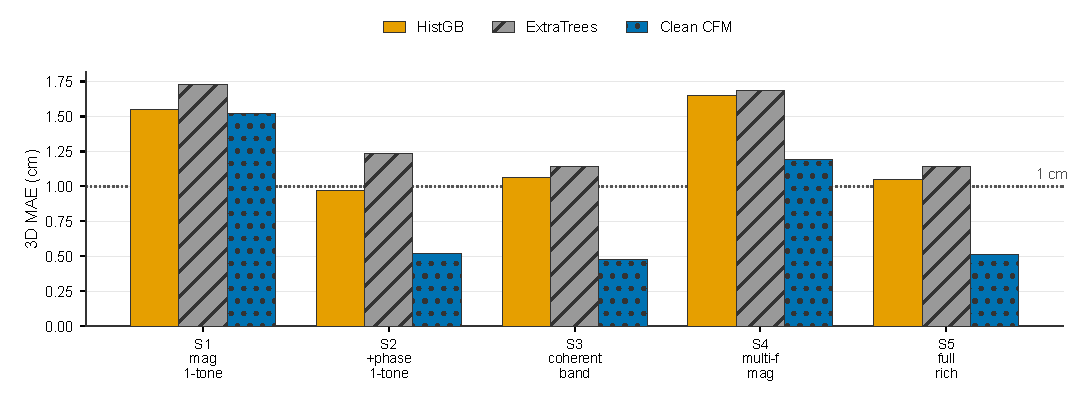
\includegraphics[width=0.9\linewidth]{figures/fig_deployability.pdf}
\caption{Grouped-bar view of the feature-deployability ablation. Phase
information at one tone or across the coherent sub-band ${\sim}$402--405\,MHz moves CFM into the
sub-cm regime and gives the tree models a clear phase benefit (ExtraTrees and
HistGB improve, though not all reach sub-cm); additional magnitude-only bandwidth
does not. \textbf{Simulation.}}
\label{fig:deployability}
\end{figure}

\subsection{Geometry ablation: receiver placement sets localizability, and the posterior reports it}\label{sec:res-modality}
Localization quality is ultimately set by \emph{where the receivers are}: a
four-receiver array makes a coordinate recoverable only if the receivers break
the symmetry along that axis. We make this concrete with a controlled
receiver-geometry ablation and ask not only ``how accurate?'' but ``does the
estimator report when an axis is unrecoverable?'' We compare two arrays
(Fig.~\ref{fig:geom-ablation}): a
\emph{mirror-symmetric} array with all four receivers in the $y=0$ plane (so the
forward operator is invariant to $y\!\to\!-y$ and the $y$ coordinate is
unobservable by construction), and the main anti-symmetric side-wall array, whose
$\pm x/\pm z$ wall placement breaks that symmetry and recovers $y$. This is why
geometry matters in localization, and it is the regime in which a
\emph{point} estimator is misleading: when two positions (a coordinate and its
mirror) explain the measurement equally well, a single point silently picks one.

A generative posterior, by contrast, can represent \emph{both} hypotheses. On the
mirror-symmetric array the CFM posterior is genuinely \emph{bimodal}
(Fig.~\ref{fig:bimodal}): it captures
the true position's mirror partner in $49.7\%$ of high-$|y|$ cases and attains
joint $90\%$ coverage $0.946$, while the 3D point error sits at the
${\sim}\SI{2.5}{cm}$ unobservable-$y$ floor---the posterior mean falls
\emph{between} the two modes, which is exactly why a single point estimate is
misleading here. The competing probabilistic methods
fail to represent the ambiguity in opposite ways: a 2-component mixture-density
network \emph{covers but does not split} (it widens into one blob), and the deep
ensemble \emph{collapses} (joint $90\%$ coverage $0.017$, zero mirror capture).
On the anti-symmetric side-wall array the same CFM posterior is \emph{unimodal},
because the geometry makes $y$ observable in simulation. Posterior
\emph{modality} therefore tracks the invertibility of the receiver geometry
within this controlled ablation, and only the generative flow follows the
modality change faithfully. The mirror-symmetric array is a deliberate ablation
geometry, distinct from the main side-wall dataset; as Table~\ref{tab:modality-ablation}
makes explicit, the two arrays also differ in feature representation (4-D
magnitude-only RSSI for the symmetric array versus the 180-D rich vector for
the main array), so this is not a feature-matched comparison. The bimodality is
nonetheless attributable to geometry rather than feature richness: the
mirror-symmetric forward map is invariant to $y\!\to\!-y$ \emph{by construction},
so $y$ is unobservable for any feature set, and a richer feature vector cannot
remove an exact geometric symmetry.

\begin{figure}[t]
\centering
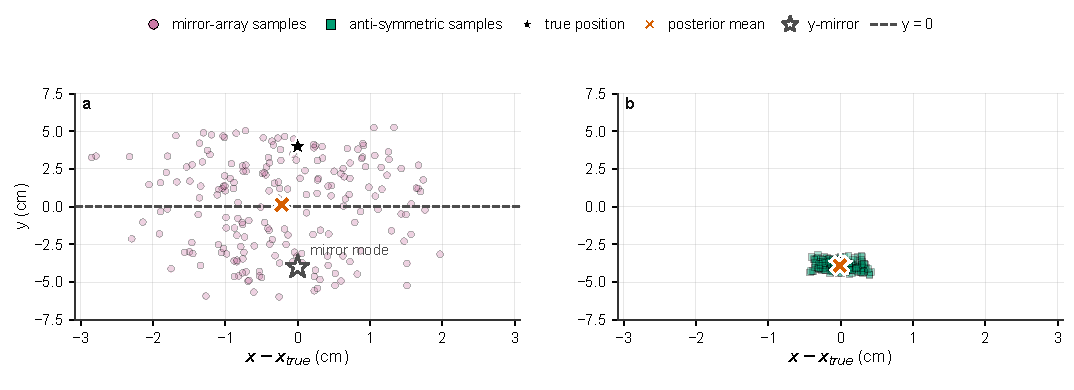
\includegraphics[width=\linewidth]{figures/fig_bimodal.pdf}
\caption{Posterior modality tracks receiver-geometry invertibility, shown with
real CFM samples for a high-$|y|$ test point (the $x$--$y$ plane). \emph{Left:} on
the mirror-symmetric array the posterior is \emph{bimodal}---it places mass on
both the true position and its $y$-mirror, so the posterior mean falls between the
modes and the point estimate is misleading. \emph{Right:} on the anti-symmetric
side-wall array the posterior for a comparable high-$|y|$ point is \emph{unimodal}
and concentrated on the truth (note the shared $y$-scale). \textbf{Simulation.}}
\label{fig:bimodal}
\end{figure}

\begin{table*}[t]
\centering
\caption{Self-contained receiver-array modality ablation. The mirror-symmetric row tests an intentionally non-invertible $y$ geometry; the anti-symmetric side-wall row is the corrected-geometry initial-stage subset run used to establish the unimodal comparator. \textbf{Simulation.}}
\label{tab:modality-ablation}
\scriptsize
\setlength{\tabcolsep}{3pt}
\begin{tabular}{@{}p{0.16\linewidth}p{0.25\linewidth}p{0.17\linewidth}cccc@{}}
\toprule
Array & Dataset and feature dimension & CFM configuration & Samples & Mirror capture & Joint 90\% & 3D point error \\
 & & & & (\%) & coverage & (cm) \\
\midrule
Mirror-symmetric array & $4$-D RSSI ablation dataset; all sensor $y$ values are $0.0$ & no-OT, no-EMA, Euler; $600$ epochs & $300$ & $49.7$ & $0.946$ & $2.546$ \\ % source: experiments/uq_bakeoff/ambiguous_bakeoff_full_20260529_033119.json:5-24,33-43; reports/stage2_y_observability/uncertainty_bakeoff_design.md:120-140
Anti-symmetric side-wall array & Initial-stage subset ($N=1980$); $180$-D rich features & no-OT, EMA $0.999$, Euler; $600$ epochs & $200$ & $0.0$ & $0.856$ & $0.501$ \\ % source: experiments/uq_bakeoff/cfm_uq_score_20260528_234224.json:410-430; reports/stage2_y_observability/uncertainty_bakeoff_design.md:63,146-148
\bottomrule
\end{tabular}
\end{table*}

\begin{figure}[t]
\centering
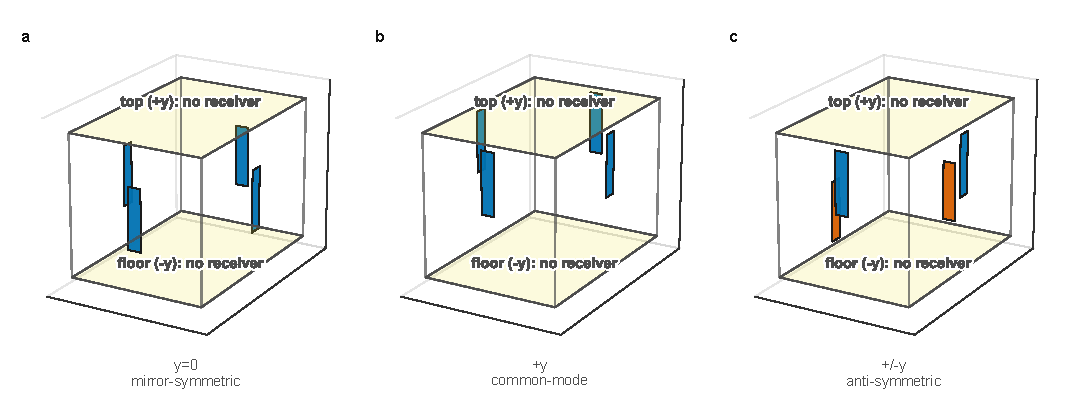
\includegraphics[width=\linewidth]{figures/fig_geometry_ablation.pdf}
\caption{Receiver-placement ablation, drawn with $y$ (height) vertical; the
shaded $\pm y$ top/floor faces carry no receiver and only the receiver
\emph{height} ($y$-coordinate) changes between panels. (a)~Mirror-symmetric
array with all four receivers at the same height ($y=0$): the forward map is
invariant to $y\!\to\!-y$, so $y$ is unobservable and the CFM posterior is
bimodal. (b)~Common-mode shift ($+y$): weak, biased $y$ information. (c)~The
main side-wall array places the receivers anti-symmetrically in height (green
upper, orange lower), breaking the symmetry so that $y$ becomes observable and
the posterior is unimodal. \textbf{Simulation.}}
\label{fig:geom-ablation}
\end{figure}

\subsection{Posterior width carries orientation uncertainty}\label{sec:res-orient}
On the main dataset, changing only the capsule's orientation at a fixed position
moves the RF fingerprint more than physically relocating the capsule does
(within-position-across-pose spread ratio ${\approx}1.17$--$1.22$). The backbone
absorbs this by invariance: the per-pose systematic bias is tiny (weighted-RMS
$x/y/z = 0.027/0.005/0.046\SI{}{cm}$, all below \SI{0.05}{cm} per axis;
maximum signed bias \SI{0.074}{cm}), and a
$180^\circ$ flip about $y$ does not flip the $y$ estimate. The orientation-induced
spread of the point estimate is small in the mean ($x/y/z/\text{3D} =
0.123/0.145/0.187/0.320\SI{}{cm}$) but has a heavy tail (max 3D \SI{3.25}{cm}).
Critically, the posterior \emph{width} tracks that orientation-induced spread at
Spearman $\rho = 0.748/0.826/0.828$ ($x/y/z$; 3D $0.847$), and the
orientation-marginal posterior (pooling a position's poses) is
$1.20$--$1.36\times$ wider than the pose-conditioned posterior while covering
$100\%$ of the per-pose cloud---a conservative representation of unknown pose.
As a diagnostic, pose is a five-way classification problem (random-forest
accuracy $74.9\%\pm2.5\%$ vs $20\%$ chance): the out-of-plane $z90/x90$ poses are
perfectly separable (recall $1.00$) while the in-plane $y$-family
$\{\text{identity},y90,y180\}$ is degenerate (recall $0.55$--$0.61$)---the
orientation-space mirror of the $y$-position blind spot. Only five axis-aligned
poses are sampled, so this ``orientation-marginal'' is a five-sample
approximation, not a true $SO(3)$ marginal (Section~\ref{sec:discussion}).
Figure~\ref{fig:orient} confirms that marginalizing unknown pose widens the
posterior while conservatively covering the fixed-position pose cloud.

\begin{figure}[t]
\centering
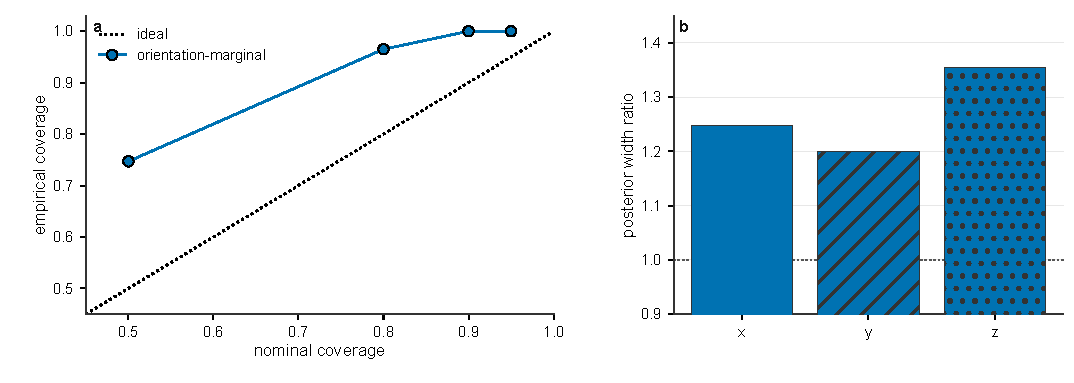
\includegraphics[width=0.9\linewidth]{figures/fig_orient.pdf}
\caption{Orientation-marginal uncertainty on the main dataset. The left panel
shows empirical coverage of the fixed-position pose cloud by the
orientation-marginal posterior; the right panel shows that marginalizing unknown
pose widens the posterior relative to pose-conditioned sampling. \textbf{Simulation.}}
\label{fig:orient}
\end{figure}
